%!TEX root = main.tex
%!TEX encoding = UTF-8 Unicode

\appendix
\part{Appendix 附录}
\chapter[矢量代数]{Vector calculus 矢量代数}\label{appendix.A}
物理中常用三个数$ \begin{pmatrix}
x \\ y \\ z
\end{pmatrix}$来描述一个东西的位置。我们将其称作矢量$\vec{v}$,在它头上放了一个箭头。这三个数称作矢量沿三个坐标轴的分量。第一个数说了这个矢量沿$x$方向走了多远,第二个是沿$y$方向以及第三个是沿$z$方向。例如,$\vec{w}= \begin{pmatrix}
0 \\ 4 \\ 0
\end{pmatrix}$是一个指向$y$轴方向的矢量。

\marginpar{
	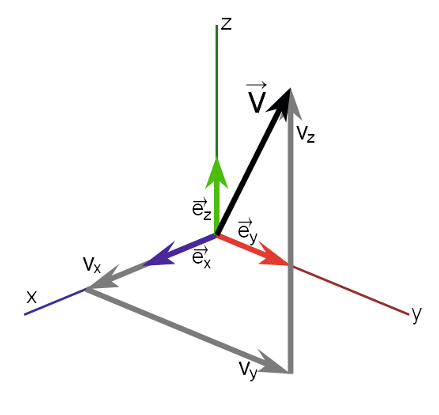
\includegraphics[width=.4\textwidth]{Figure/fig_appendix_A_1.png}
}

矢量间可以相加
\begin{equation}
\vec{v} = \begin{pmatrix}
v_x \\ v_y \\ v_z
\end{pmatrix} \quad
\vec{w} = \begin{pmatrix}
w_x \\ w_y \\ w_z
\end{pmatrix} \quad \rightarrow \quad
\vec{v}+\vec{w}= \begin{pmatrix}
v_x+w_x \\ v_y+w_y \\ v_z+w_z
\end{pmatrix}
\end{equation}
也可以相乘
\begin{equation}
\vec{v}\cdot\vec{w} = \begin{pmatrix}
v_x \\ v_y \\ v_z
\end{pmatrix} \cdot \begin{pmatrix}
w_x \\ w_y \\ w_z
\end{pmatrix} =
v_xw_x +v_yw_y +v_zw_z\text{。}
\end{equation}

乘法的结果是一个数($=$标量)而不是矢量,其有特定的名称:{标量积(scalar product)}。计算矢量与自身的标量积可以得到其长度:
\begin{equation}
\text{长度}(\vec{v}) = \sqrt{\vec{v}\cdot\vec{v}}\text{。}
\end{equation}
注意并不是随便三个量都可以写在一起,用括号包起来,作为一个矢量。例如,把一个房间里的温度$T$,压强$P$和湿度$H$放在一起:
\begin{equation}
\begin{pmatrix}
T \\ P \\ H
\end{pmatrix}\text{。}
\end{equation}
没人阻止我们把他们放在一起,但这结果毫无意义,而且显然不是一个矢量,因为不存在能将它们混在一起的线性关系。而如果我们仅仅是换一个视角\footnote{译注:本意,即视线的角度。}去考察一个矢量,它的坐标分量将会互相转换%
\mpar{这一点等会儿会有更清楚的说明。}%
。故将这些坐标分量写在一起用括号包起来是有用的。另外,如果分量会因视角的改变而发生混合的话,将其写成位置矢量的形式是有用的。

从现在开始,我们将完全按照位置矢量$\vec{v}$的变换方式的量称为一个矢量。这句话的意思是,如果在某种变换下我们有$\vec{v}\rightarrow\vec{v}'=M\vec{v}$,则任何依$\vec{w}\rightarrow\vec{w}'=M\vec{w}$作变换的量都是矢量。动量和加速度是典型的例子。

物理中我们将经常碰到这种思路。当我们把一些量写在一起放在一对括号中时,它们未必是矢量,但一定是在某些线性算符下相互变换的量。线性算符常通过与矩阵的乘法来表示。

\section[基矢]{Basis Vectors 基矢}\label{appendix.A.1}
我们可以通过引入基矢来更一般的讨论沿坐标轴的分量这件事。基矢是一组线性独立%
\mpar{一组矢量$\{\vec{a},\vec{b},\vec{c}\}$被称为是线性独立的,若方程$c_1\vec{a}+c_2\vec{b}+c_3\vec{c}=0$成立当且仅当$c_1=c_2=c_3=0$。这说的其实就是其中任何一个矢量不能表达为其他矢量的线性组合:如果有$c_1\vec{a}+c_2\vec{b}+c_3\vec{c}=0$对非零的系数成立,则有$c_1\vec{a}+c_2\vec{b}=-c_3\vec{c}$。}%
且长度为一%
\footnote{译注:一般资料上并不要求最后一条;满足这一条的称为单位基矢。}%
的矢量。三维里我们需要三个基矢,从而能将任何矢量都用基矢量的组合来表达。一个简单的选择是:
\begin{equation}
\vec{e}_1 = \begin{pmatrix}
1 \\ 0 \\ 0
\end{pmatrix}\text{,}\quad
\vec{e}_2 = \begin{pmatrix}
0 \\ 1 \\ 0
\end{pmatrix} \text{,}\quad
\vec{e}_3 = \begin{pmatrix}
0 \\ 0 \\ 1
\end{pmatrix}
\end{equation}
这样任意三维矢量$\vec{v}$都能用基矢表出
\begin{equation}
\vec{v} = \begin{pmatrix}
v_x \\ v_y \\ v_z
\end{pmatrix} = v_1\vec{e}_1 + v_2\vec{e}_2 + v_3\vec{e}_3 =
v_1 \begin{pmatrix}
1 \\ 0 \\ 0
\end{pmatrix}+
v_2  \begin{pmatrix}
0 \\ 1 \\ 0
\end{pmatrix} +
v_3  \begin{pmatrix}
0 \\ 0 \\ 1
\end{pmatrix}\text{。}
\end{equation}
$v_1,v_2,v_3$三个数叫做$\vec{v}$的分量。注意分量是依赖于基矢的。

前面提到的矢量\mpar{$\vec{w}= \begin{pmatrix}
0\\4\\0
\end{pmatrix}$}$\vec{w}$由此可以写成$\vec{w}= 0\vec{e}_1 + 4\vec{e}_2 + 0\vec{e}_3$。对基矢另一个同样好的选法是
\begin{equation}
\tilde\vec{e}_1 = \frac{1}{\sqrt{2}} \begin{pmatrix}
1 \\ 1 \\ 0
\end{pmatrix}\text{,}\quad
\tilde\vec{e}_2 = \frac{1}{\sqrt{2}} \begin{pmatrix}
1 \\ -1 \\ 0
\end{pmatrix} \text{,}\quad
\tilde\vec{e}_3 = \begin{pmatrix}
0 \\ 0 \\ 1
\end{pmatrix}\text{。}
\end{equation}
在这组基下矢量$\vec{w}$看起来会有点不同:
\begin{equation}
\vec{w}= 2\sqrt{2}\tilde\vec{e}_1 -2\sqrt{2}\tilde\vec{e}_2 + 0\tilde\vec{e}_3
= 2\sqrt{2} \frac{1}{\sqrt{2}} \begin{pmatrix}
1 \\ 1 \\ 0
\end{pmatrix}-2\sqrt{2}
\frac{1}{\sqrt{2}} \begin{pmatrix}
1 \\ -1 \\ 0
\end{pmatrix} =\begin{pmatrix}
0\\4\\0
\end{pmatrix} \text{。}
\end{equation}
从而将$\vec{w}$用在新基矢下的分量写出
\[
\tilde\vec{w} = \begin{pmatrix}
2\sqrt{2} \\ -2\sqrt{2} \\ 0
\end{pmatrix}\text{。}
\]
这并不是一个不同的矢量,而只是一个不同的描述!准确地讲,$\tilde\vec{w}$是原坐标系中的矢量$\tilde\vec{w}$在一个相对有旋转的坐标系下描述。%
\footnote{译注:在整个附录\ref{appendix.A}里作者就没说过几句准确的话,这句话也说得挺糙的。}

\section[坐标系变换]{Change of Coordinate Systems 坐标系变换}\label{appendix.A.2}
通过矩阵,我们可以更精确地描述不同坐标系间的联系。两个不同的坐标系可以代表实验中两个持不同视角的观察者,或者仅仅是{\bf 一个}想使用一套新的基矢的观察者。这些描述之间的关系是什么?为了避免复杂的讨论,让我们假定这两个坐标系的原点和$z$轴都是一样的。这样的话就只是$x$和$y$轴有区别了。进一步假定实验中某个重要的量用矢量$\vec{v}$描述。

如果第一个观察者看到的是矢量$\vec{v}= \begin{pmatrix}
v_x \\ v_y \\ v_z
\end{pmatrix}$,我们能通过三角函数$\sin(\phi)$,$\cos(\phi)$和$\tan(\phi)=\frac{\sin(\phi)}{\cos(\phi)}$来计算出第二个观察者看到的$\vec{v}= \begin{pmatrix}
v_{x'} \\ v_{y'} \\ v_{z'}
\end{pmatrix}$,如图\ref{fig:appendix.A.1} 所示:
\marginpar{
	\figcaption{矢量在两个不同的坐标系下分量的示意图。细节见正文。}
	\label{fig:appendix.A.1}
}

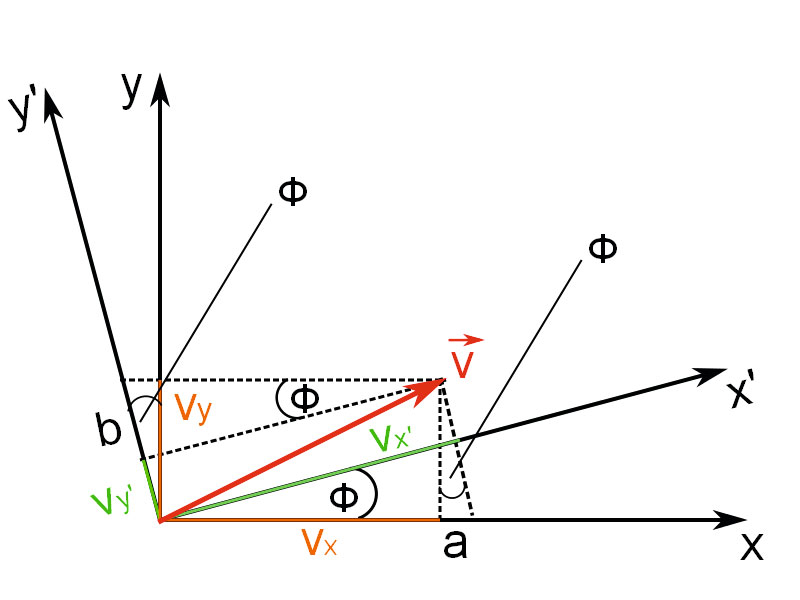
\includegraphics[width=\textwidth]{Figure/fig_appendix_A_3.png}

计算$v_x$和$v_{x'}$的关系,由
\[
\cos(\phi)=\frac{v_{x'}}{v_x+a} \rightarrow v_{x'}=(v_x+a)\cos(\phi)
\]
以及
\[
\tan(\phi)=\frac{a}{v_y}\rightarrow a=v_y\tan(\phi)\text{。}
\]
得到
\[
\begin{aligned}
v_{x'}=(v_x+v_y\tan(\phi))\cos(\phi)&=\left(v_x+v_y\frac{\sin(\phi)}{\cos(\phi)}\right)\cos(\phi) \\
 & = v_x\cos(\phi)+v_y\sin(\phi)\text{。}
\end{aligned}
\]
类似的,利用
\[
\cos(\phi) = \frac{v_y}{v_{y'}+b}\rightarrow v_{y'}=v_y\frac{1}{\cos(\phi)}-b
\]
和
\[
\tan(\phi)=\frac{v_y}{v_{y'}+b}\rightarrow b=v_{x'}\tan(\phi)
\]
再借助$\sin^2(\phi)+\cos^2(\phi)=1$导出
\[\begin{split}
v_{y'}&=v_y\frac{1}{\cos(\phi)}-v_{x'}\tan(\phi)=v_y\frac{1}{\cos(\phi)}-(v_x\cos(\phi)+v_y\sin(\phi))\frac{\sin(\phi)}{\cos(\phi)}  \\
&= v_y\frac{\sin^2(\phi)+\cos^2(\phi)}{\cos(\phi)}-v_x\sin(\phi)-v_y\frac{\sin^2(\phi)}{\cos(\phi)} = v_y\cos(\phi)-v_x\sin(\phi)
\end{split}\]
最终有$v_{y'}=-v_x\sin(\phi)+v_y\cos(\phi)$。

我们能将其用一个旋转矩阵来表达:
\begin{equation}
\begin{aligned}
\begin{pmatrix}
v_{x'} \\ v_{y'} \\ v_{z'}
\end{pmatrix} &= R_z(\phi)\vec{v} =
\begin{pmatrix}
\cos(\phi) & \sin(\phi) & 0 \\
-\sin(\phi) & \cos(\phi) & 0 \\
0 & 0 & 1
\end{pmatrix}
\begin{pmatrix}
v_x \\ v_y \\ v_z
\end{pmatrix} \\
&= \begin{pmatrix}
\cos(\phi)v_x+\sin(\phi)v_y \\ -\sin(\phi)v_x+\cos(\phi)v_y \\ v_z
\end{pmatrix}\text{。}
\end{aligned}
\end{equation}
将矩阵的每一行与未旋转的矢量相乘,便得到了旋转后的矢量。如之前所提到的,沿$z$轴的分量$v_3$对于不同的观察者而言是相同的。矩阵$R_z(\phi)$描述了一个绕$z$轴转动了角度$\phi$的旋转。

\section[矩阵乘法]{Matrix Multiplication 矩阵乘法}\label{appendix.A.3}
像这样通过矩阵来作计算是一个极大的简化。矩阵乘法的规则就是行乘列。如果将一个矢量看做一个一列三行的矩阵(一个$3\times 1$矩阵),则标量积也可以看做是矩阵乘法的一种特殊情况。即
\begin{equation}
\vec{v}\cdot\vec{w} = \vec{v}^T\vec{w}= \begin{pmatrix}
v_x & v_y & v_z
\end{pmatrix} \begin{pmatrix}
w_x \\ w_y \\ w_z
\end{pmatrix} = v_xw_x +v_yw_y +v_zw_z\text{,}
\end{equation}
其中$T$代表转置,即行变成列,列变成行。那么$\vec{v}^T$便是一个$1$行$3$列的矩阵。这样写的话标量积就也成了行乘列的矩阵乘法。

类似的,两个矩阵的乘法也就是左边矩阵的每一行乘右边矩阵的每一列,如图\ref{fig:appendix.A.2}。下面是一个具体的例子

\marginpar{
	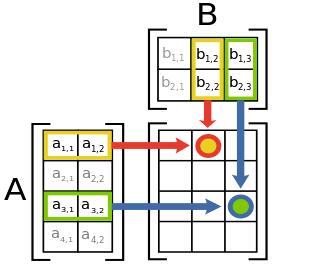
\includegraphics[width=.4\textwidth]{Figure/fig_appendix_A_4.png}
	\figcaption{矩阵乘法示意图。时时刻刻记住{\bf 行乘列}。第一个指标代表所在的行数,第二个代表列数。在例子中,乘积矩阵红色的元素$c_{1,2}=a_{1,1}b_{1,2}+a_{1,2}b_{2,2}$,蓝色的元素$c_{3,3}=a_{3,1}b_{1,3}+a_{3,2}b_{2,3}$。一般的,$c_{i,j}=a_{i,k}b_{k,j}=a_{i,1}b_{1,j}+a_{i,2}b_{2,j}+\dots$ Figure by Olivier Perrin (Bilou Wikimedia Commons) released under a CC BY-SA 3.0 licence: \url{http://creativecommons.org/licenses/by-sa/3.0/deed.en}. URL: \url{http://commons.wikimedia.org/wiki/File:Matrix_multiplication_diagram_2.svg}, Accessed: 28.1.2015}
	\label{fig:appendix.A.2}
}

\begin{equation}
\begin{aligned}
M= \begin{pmatrix}
2 & 3 \\ 1 & 0
\end{pmatrix} \quad N =
\begin{pmatrix}
0 & 1 \\ 4 & 8
\end{pmatrix} \\
MN = \begin{pmatrix}
2 & 3 \\ 1 & 0
\end{pmatrix}
\begin{pmatrix}
0 & 1 \\ 4 & 8
\end{pmatrix} =
\begin{pmatrix}
2\cdot 0+3\cdot 4 & 2\cdot 1+3\cdot 8 \\ 1\cdot 0+0\cdot 4 & 1\cdot 1+0\cdot 8
\end{pmatrix} =
\begin{pmatrix}
12 & 26 \\ 0 & 1
\end{pmatrix}
\end{aligned}
\end{equation}
时刻把{\bf 行乘列}记在脑子里\footnote{译注:说起来,什么是行什么是列也是一个需要记牢的东西,尤其是与台湾友人交流时。}。注意两个矩阵的乘法是不对易的,即一般来说$MN\ne NM$。

\section[标量]{Scalars 标量}\label{appendix.A.4}
另一个值得注意的事情是,两个矢量标量积的结果对于所有观察者而言都是相同的。这看起来可以作为标量的定义:标量是对于全部观察者都相同的量。这不只是简单的在说每一个数都是标量,因为矢量的每一个分量都是一个数,但是它们对于不同的观察者而言却不一样。作为对比,两个矢量的标量积对于全体观察者却是相同的。这源于,矢量的长度与其与自身的标量积直接相关这一事实。改变观察的视角或位置并不会改变任何东西的长度。矢量的长度被称作旋转下的不变量,即无论我们怎样旋转系统其都保持原样。

\section[左手/右手坐标系]{Right-handed and Left-handed Coordinate Systems 左手/右手坐标系}\label{appendix.A.5}
当我们谈论两个观察者时,我们默认了它们对坐标系的定义都是相同的。而事实上,我们有两种可能的选择,它们这是依旧能通过矩阵乘法相联系,却不能靠转动了。两个观察者可能是一个选择了所谓的右手坐标系,而另一个选择了左手坐标系。

\marginpar{
	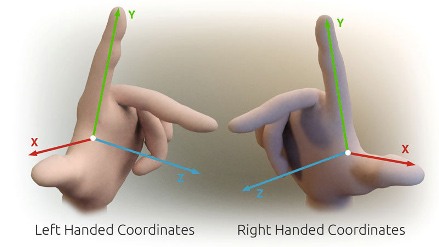
\includegraphics[width=.4\textwidth]{Figure/fig_appendix_A_5.png}
	\figcaption{右手坐标系和左手坐标系。 Figure by Primalshell (Wikimedia Commons) released under a CC-BY-SA-3.0 licence: \url{http://creativecommons.org/licenses/by-sa/3.0/deed.en}. URL:\url{http://commons.wikimedia.org/wiki/File:3D_Cartesian_Coodinate_Handedness.jpg}, Accessed: 1.12.2014}
}

我们无法将一个左手系旋转成一个右手系。事实上,这两类坐标系通过镜面反射相关联。这就是说,右手系和左手系由如下形式的变换相联系%
\footnote{译注:原文这里给出的其实是一个相对原点的反射,而不是镜面反射。当然,这两种反射之间只差一个转动。}
\begin{equation}
\begin{pmatrix}
v_1 \\ v_2 \\ v_3
\end{pmatrix} \rightarrow
\begin{pmatrix}
-v_1 \\ -v_2 \\ -v_3
\end{pmatrix}\text{,}
\end{equation}
就是说把全部空间坐标都反一个号。人们也习惯于将这类变换称作{\bf 宇称变换(parity transformation)}。我们可以用如下方式来表示一个宇称变换
\begin{equation}
\vec{v} \rightarrow \vec{v}' = P\vec{v} = \begin{pmatrix}
-1 & 0 & 0 \\ 0 & -1 & 0 \\ 0 & 0 & -1
\end{pmatrix}
\begin{pmatrix}
v_1 \\ v_2 \\ v_3
\end{pmatrix} =
\begin{pmatrix}
-v_1 \\ -v_2 \\ -v_3
\end{pmatrix}\text{。}
\end{equation}

\chapter[微积分]{Calulus 微积分}\label{appendix.B}

\section[Product Rule]{Product Rule 莱布尼兹律}\label{appendix.B.1}
莱布尼兹律\footnote{译注:直译为“乘积规则”,鉴于这种叫法在中文文本中较罕见,故译作“莱布尼兹律”。}
\begin{equation}
\frac{\rd}{\rd x} \left(f(x)g(x)\right) = \left(\frac{\rd f(x)}{\rd x}\right) g(x) + f(x) \left(\frac{\rd g(x)}{\rd x}\right) \equiv f'g + fg'
\label{equB.1}
\end{equation}
可直接由导数的定义得到
\begin{equation*}
\begin{aligned}
\frac{\rd}{\rd x} \left[f(x)g(x)\right] &= \lim_{h\rightarrow 0} \frac{f(x+h)g(x+h)-f(x)g(x)}{h} \\
 &= \lim_{h\rightarrow 0} \frac{\left[f(x+h)g(x+h)-f(x+h)g(x)\right]+\left[f(x+h)g(x)-f(x)g(x)\right]}{h} \\
 &= \lim_{h\rightarrow 0}{f(x+h)\frac{g(x+h)-g(x)}{h} +g(x)\frac{f(x+h)-f(x)}{h}} \\
 &= f(x)g'(x)+g(x)f'(x)
\end{aligned}
\end{equation*}
\section[分部积分]{Integration by Parts 分部积分}\label{appendix.B.2}
\begin{quote}
据说, Peter Lax 被授予美国国家科学奖章时,其他获奖人(可能不是数学家)问他凭借什么拿到的这个奖。 Lax 回答:“我做了个分部积分。” \\
- Willie Wrong\mpar{是他在\url{www.math.stackexchange.com}上说的。}
\end{quote}

从莱布尼兹律可以直接得到一个重要的积分手段。将莱布尼兹律一式积分%
\mpar{见\ref{equB.1}式,并利用微积分基本定理$\int_a^b h'(x)=h(b)-h(a)$。}
\begin{equation}
\underbrace{\int_a^b \rd x\, \frac{\rd}{\rd x}\left(f(x)g(x)\right)}_{=\left.f(x)g(x)\right|_a^b} = \int_a^b\rd x\, \left(\frac{\rd f(x)}{\rd x}\right)g(x) + \int_a^b\rd x\, f(x)\left(\frac{\rd g(x)}{\rd x}\right)
\end{equation}
移项,得到
\begin{equation}
\int_a^b \rd x\, \left(\frac{\rd f(x)}{\rd x}\right)g(x) = \left.f(x)g(x)\right|_a^b - \int_a^b\rd x\, f(x)\left(\frac{\rd g(x)}{\rd x}\right)\text{。}
\label{equB.3}
\end{equation}
当讨论场的物理时,这个手段很是有用:在全空间作积分时,即$a=-\infty,b=\infty$,由于一切场量在无穷远处都必须为零%
\mpar{\ref{sec2.4}节中我们说到了没什么能比光速还快,故无穷远处的场一定不会对有限$x$处的物理产生影响。}%
,边界项为零$\left.f(x)g(x)\right|_a^b=0$。

\section[Taylor 级数]{The Taylor Series\quad Taylor 级数}\label{appendix.B.3}
Taylor 级数使我们能将任何无穷阶可微函数写成幂级数形式
\begin{equation}
f(x) = f(a) + (x-a)f'(a) + \frac{1}{2}(x-a)^2f''(a)+\dots
\end{equation}
\begin{itemize}
\item 一方面我们能用它来求某些函数的级数形式。这可以用来,例如,说明$\ue^{\ri x}=\cos (x)+\ri\sin (x)$。
\item 另一方面,也能用它来得到函数在某点附近的近似值。当出于某些原因我们可以略去高阶项,不用考虑无穷多项时,这公式的用处会很大。比如说我们要算函数$f(x)$在$y$的邻域中一点$y+\Delta y$的值,可以写出%
\mpar{不要被这些变量的名字搞混了。上面的公式里我们是从$a$出发计算函数在$x$处的值。而这里我们是希望利用$y$处的信息来得到$f$在$y+\Delta y$处的性质。准确的关系是:$x=y+\Delta y$和$a=y$。}
\end{itemize}
\begin{equation}
f(y+\Delta y) = f(y)+(y+\Delta y-y)f'(y)+\dots =f(y)+\Delta y f'(y)+\dots
\end{equation}
这就是说,通过在$y$处函数的性质,我们能得到其在$y+\Delta y$处的近似值。对于无穷小邻域%
\footnote{\textcolor{red}{译注:原文有误,已更正。}}%
$\Delta y=\epsilon\rightarrow 0$的极端情况,函数的改变量可以仅用 Taylor 级数的一(线性)项来表示
\begin{equation}
\Delta f =f(y+\epsilon)-f(y)=f(y)+\epsilon f'(y)+\dots -f(y)=\epsilon f'(y) + \underbrace{\dots}_{\mathclap{\approx 0\text{由于}\epsilon^2\approx 0}}
\end{equation}

这个式子是最有用的数学工具之一,它也能通过微积分基本定理和分部积分推出来。基本定理说
\begin{equation}
\int_a^x\rd t\, f'(t) = f(x) - f(a) \rightarrow f(x)=f(a)+\int_a^x\rd t\, f'(t)\text{。}
\end{equation}
可以将第二项用分部积分写开:在$f'(t)$前面补一个$1$成$1f'(t)$,利用\ref{equB.3}式取$g'(t)=1$的情况。分部积分能改写积分%
\mpar{\textcolor{red}{译注:原文有误,已更正。}}%
$\int_a^b v'u = \left.vu\right|_a^b-\int_a^b vu'$,积掉一项而对另一项微分。这里我们积$g'(t)=1$而微分$f'(t)$,即式子里$g'=v'$及$f'=u$。求得
\begin{equation}
f(x) = f(a)+\int_a^x\rd t\, f'(t) = f(a) + \left.g(t)f(t)\right|_a^x - \int_a^b \rd t g(t)f''(t) \text{。}
\end{equation}

现在的问题是$g(t)$是啥。我们目前只知道$g'(t)=1$,但却有无穷多个函数的导数都是这个:对于任意常数$c$,函数$g=t+c$都满足$g'(t)=1$。我们选取%
\mpar{方程对任意$c$都成立,我们自然可以随便选一个,但那样就推不出我们想要的公式了。选取恰当的$c$是为了得到一个有用的关于$f(x)$的公式。否则$f(x)$将会同时出现在等式两侧。}%
$g=t-x$,即将积分上界的负值$-x$作为我们的常数$c$。从而上式的第二项就可以写作
\begin{equation}
\left.g(t)f(t)\right|_a^x = \left.(t-x)f(t)\right|_a^x = \underbrace{(x-x)}_{=0}f(x) -(a-x)f(a) =(x-a)f(a)
\end{equation}
从而整个式子现在写作
\begin{equation}
f(x) = f(a) + (x-a)f'(a)+\int_a^x\rd t\, (x-t)f''(t)\text{。}
\end{equation}
对最后一项再次使用分部积分,现在是%
\mpar{注意$v='(x-t)$对$t$的积分会出一个符号:$v=-(x-t)^2+d$积分常数$d$取作零。}
$v'=(x-t)$和$u=f''(t)$:
\begin{equation}
\rightarrow \int_a^x \rd t\, \underbrace{(x-t)}_{\mathclap{=v'}}\underbrace{f''(t)}_{=u} = \left.\underbrace{-\frac{1}{2}(x-t)^2}_{=v} \underbrace{f''(t)}_{=u}\right|_a^x - \int_a^x \rd t\, \underbrace{\left(-\frac{1}{2}(x-t)^2\right)}_{=v}\underbrace{f'''(t)}_{=u'}
\end{equation}
边界项同样简单的是零
\begin{equation}
\left.-\frac{1}{2}(x-t)^2f''(t)\right|_a^x = -\frac{1}{2}\underbrace{(x-x)^2}_{=0}f''(x) + \frac{1}{2}(x-a)^2f''(a)\text{。}
\end{equation}
得到公式
\begin{equation}
f(x)=f(a)+(x-a)f'(a)+\frac{1}{2}(x-a)^2f''(a)+\int_a^x \rd t\, \frac{1}{2}(x-t)^2 f'''(t)\text{。}
\end{equation}
可以继续将最后一项分部积分,但是我们应该能直接肉眼观察出规律了。Taylor 级数可以利用求和号$\Sigma$写成更紧凑的形式:
\begin{equation}
\begin{aligned}
f(x) =& \sum_{n=0}^\infty\frac{f^{(n)}(a)(x-a)^n}{n!} \\
 =& \frac{f^{(0)}(a)(x-a)}{0!} + \frac{f^(1)(a)(x-a)^1}{1!} + \frac{f^{(2)}(a)(x-a)^2}{2!} \\
 =& \frac{f^{(3)}(a)(x-a)^3}{3!}+\dots \text{,}
\end{aligned}
\end{equation}
其中$f^{(n)}$代表$f$的$n$阶导数,例如$f^{(2)}=f''$,$n!$代表$n$的阶乘,即$n!=1\cdot 2\cdot 3\dots n$。比如对$n=5$有$5!=5\cdot 4\cdot 3\cdot 2\cdot 1=120$,$2!=2\cdot 1=2$,以及定义$0!=1$。级数是下一节的主题。
\section[级数]{Series 级数}\label{appendix.B.4}
\subsection[几个重要的级数]{Important Series 几个重要的级数}\label{appendix.B.4.1}
\subsection[分裂求和]{Splitting Sums 分裂求和}\label{appendix.B.4.2}
\subsection[Einstein 求和约定]{Einstein’s Sum Convention\quad Einstein 求和约定}\label{appendix.B.4.3}

\section[指标记号]{Index Notation 指标记号}\label{appendix.B.5}
\subsection[哑指标]{Dummy Indices 哑指标}\label{appendix.B.5.1}
\subsection[带多个指标的对象]{Objects with more than One Index 带多个指标的对象}\label{appendix.B.5.2}
\subsection[对称/反对称指标]{Symmetric and Antisymmetric Indices 对称/反对称指标}\label{appendix.B.5.3}
\subsection[对称和反对称求和]{Antisymmetric $\times$ Symmetric Sums 对称和反对称求和}\label{appendix.B.5.4}
\subsection[两个重要的符号]{Two Important Symbols 两个重要的符号}\label{appendix.B.5.5}

\chapter[线性代数]{Linear Algebra 线性代数}
\section[基本的变换]{Basic Transformations 基本的变换}
\section[矩阵指数函数]{Matrix Exponential Function 矩阵指数函数}
\section[行列式]{Determinants 行列式}
\section[本征值与本征向量]{Eigenvalues and Eigenvectors 本征值与本征向量}
\section[对角化]{Diagonalization 对角化}

\chapter[其他数学概念]{Additional Mathematical
Notions 其他数学概念}
\section[Fourier 变换]{Fourier Transform\quad Fourier 变换}
\section[Delta 分布]{Delta Distribution\quad Delta 分布}
